\title{PartyMixer – Cocktails für zu Hause}
\team{%
    Kim Schenk,
    Robin Aebi}

\client{Kim Schenk,
		Robin Aebi}

\projtype{P6}

\coaches{%
	Pascal Schleuniger}

\fssummary{
Bei einer gelungenen Party darf eines auf keinen Fall fehlen, die Getränke. Diese sicherzustellen ist jedoch meistens mit viel Aufräumarbeit und Selbstaufwand verbunden. Genau da kommt der PartyMixer ins Spiel. Mit dem PartyMixer können sich die Gäste selbstständig die gewünschten Cocktails ohne Chaos oder verschüttete Getränke erstellen lassen.
}

\fsgraphics{
    \centering
\bigskip
\noindent
\begin{minipage}[t]{.4\textwidth}
\raggedright
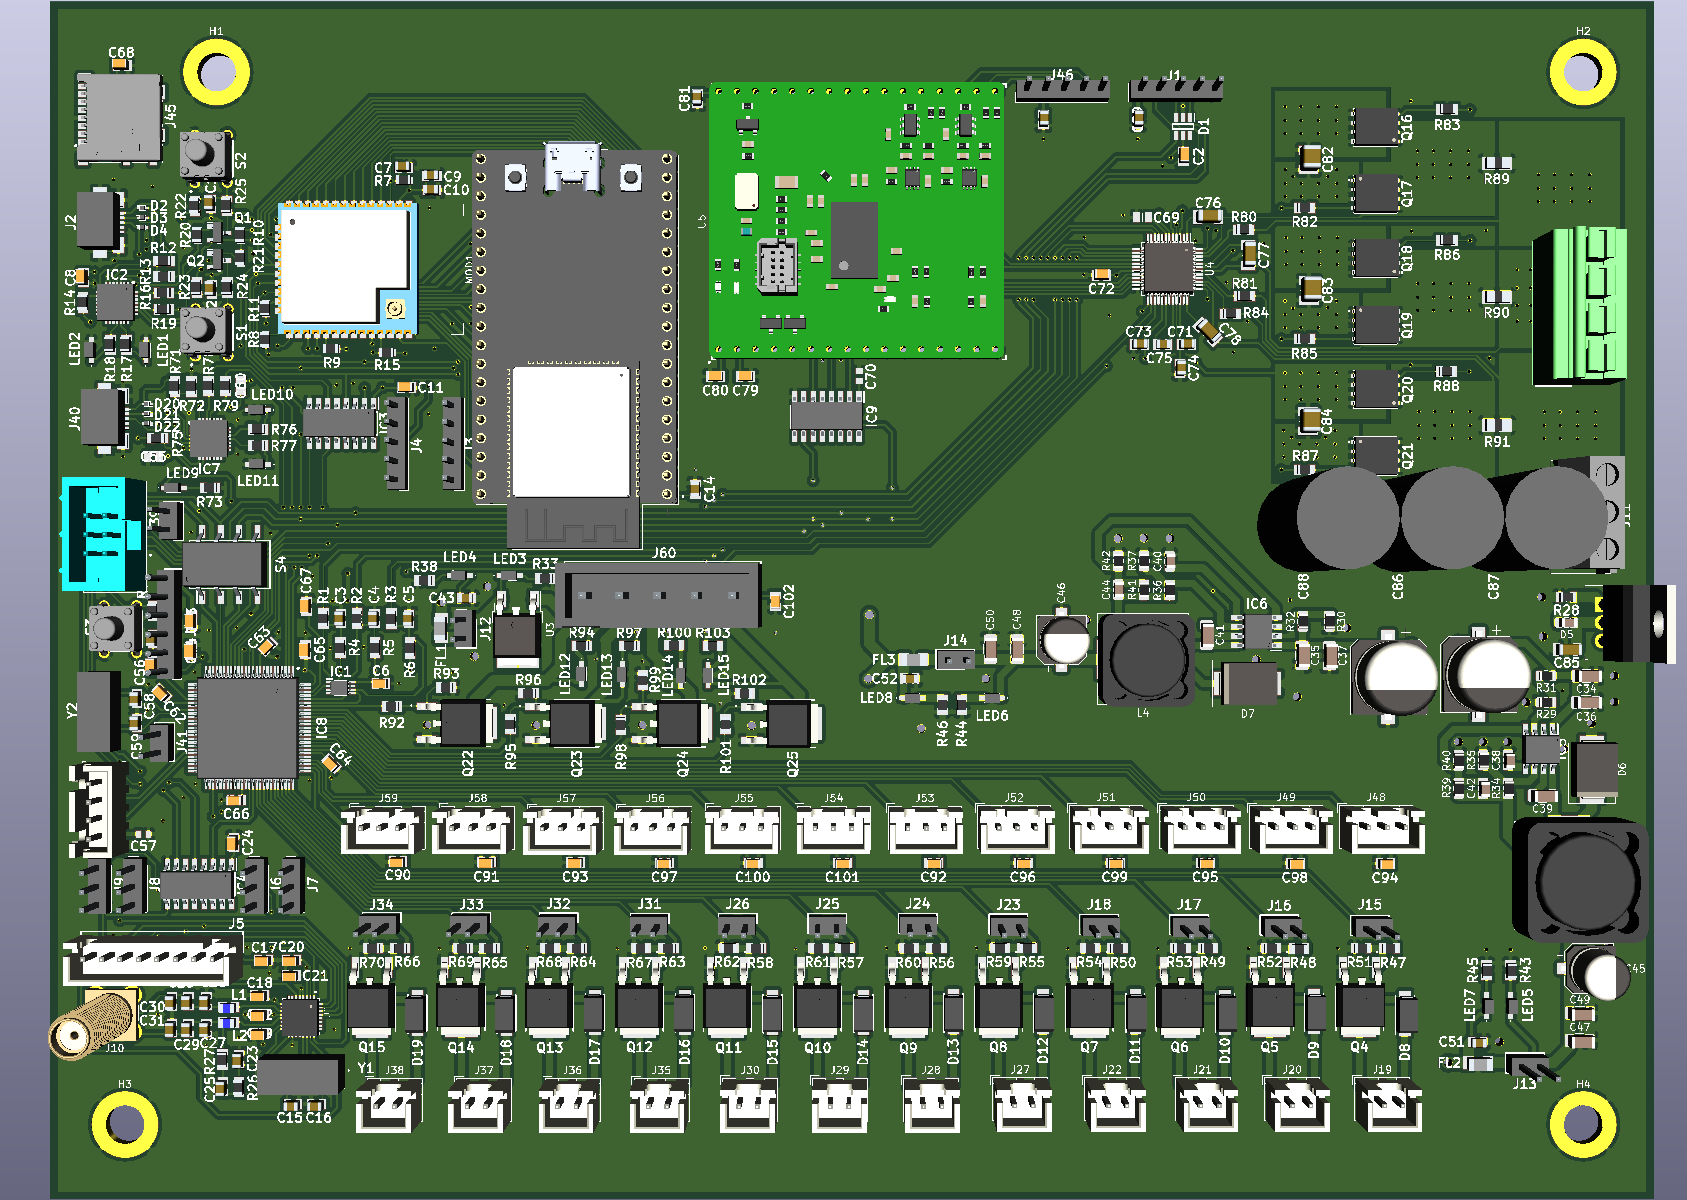
\includegraphics[height = 50mm]{images/Print_3D}\\
\graphicscaption{Print 3D-Modell}
\end{minipage}
\hfill
\noindent
\begin{minipage}[t]{.5\textwidth}
\raggedright
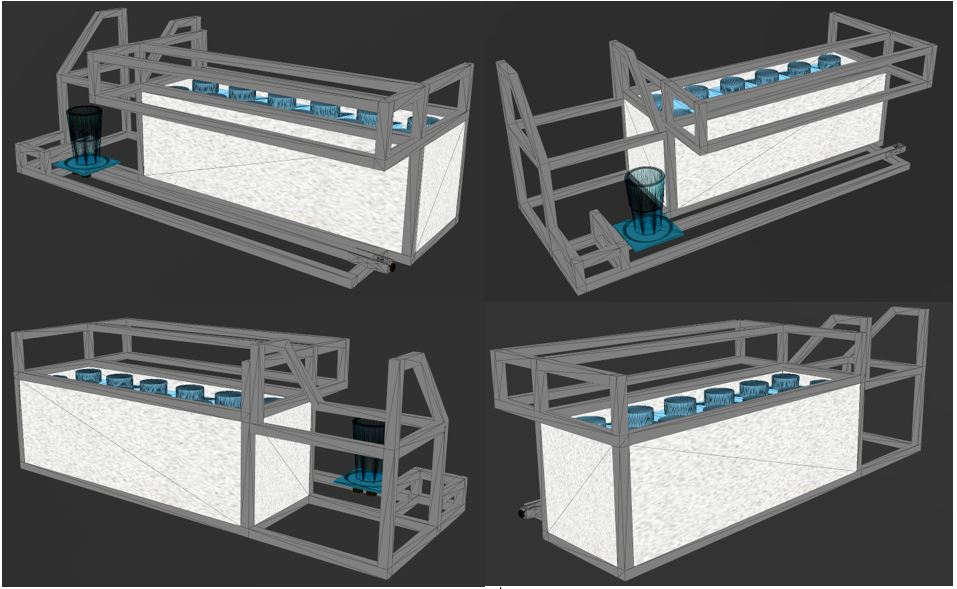
\includegraphics[height = 50mm]{images/3DModell}\\
\graphicscaption{Mechanik 3D-Modell}
\end{minipage}
}

\fscontent{
    \section{Hardware}
	Die Hardware besteht aus einer Leiterplattine, worauf alle Komponenten für die gewünschten Funtkionen enthalten sind. Dazu gehören die Speisungen, der Mikrocontroller, die Motorengruppe, das WiFi-Modul, die Ansteuerung für die Pumpen und zugehörige Sensoren und die LED-Steuerung. Ausserdem wird ein externes RFID-Modul und Display verwendet.
    \section{Software}
	Der grösste Software-Teil gehört zum Mikrocontroller. Dieser steuert die Maschine an sich. Ein weiterer Software-Teil steckt in der Android-Applikation. Darin wird das User-Interface bereitgestellt und bei Berührungen des Displays Aktionen ausgelöst. Die ausgelösten Aktionen werden im WiFi-Modul verarbeitet. Das WiFi-Modul kommuniziert dann mit dem Mikrocontroller.
    \section{Mechanik}   
    Die Mechanik ist das Skelett der Maschine. Es trägt die angesteuerten Komponenten und stellt sicher, dass die Funktion der Maschine gewährleistet ist. Zur Mechanik gehören der Rahmen, der Getränkeschlitten, die Verleidung, die Unterbringung der Elektronik und die Kühlbox. Der LED-Streifen wird auch am Rahmen befestigt.
}

\infobox{Funktionen}{%
    \footnotesize
    \setlength\tabcolsep{2pt}
    \begin{tabular}{p{0.5\textwidth}|p{0.5\textwidth}}
    \bfseries Cocktails	& \bfseries Bluetooth	\\
    Cocktails können erstellt und bearbeitet werden. & Über eine App können Cocktails erstellt und den RFID-Tags  \\
    Die Position und Art der Zutaten ist frei wählbar. & zugewiesen werden.\\
	Automatische Listenerstellung anhand der Zutaten. & \\
	 & \bfseries Datenspeicherung\\
	\bfseries Zutaten & Sämtliche Daten werden auf einer SD-Karte abgelegt.\\
	Unterscheidung Kohlesäure- und Alkoholhaltige Zutaten. & Bei einem Neustart werden die Zuletzt vorhandenen Daten\\
	Selber hinzufügen für eine breitere Cocktailauswahl. & geladen. \\
	 & \\
	\bfseries RFID & \bfseries Motor\\
	Cocktail kann einem Tag zugeordnet und ohne & Eine FOC-Regelung kontrolliert die Motorbewegungen.\\
	Suchen zubereitet werden. & \\
	 & \bfseries Mechanik\\
	\bfseries Reinigung & 12 Pumpen und Durchflusssensoren.\\
	Ein begleiteter Reinigungsmodus ist vorhanden. & Kühlbox hält Stunden kalt.\\
	 & \\
	 \bfseries Display & \\
	 Sämtliche cocktailspezifischen sowie maschinenspezifische Funtkionen können getätigt werden. & \\
    \end{tabular}
}
